\subsection{Ejercicios}
\begin{exercise}[1]
	Se pretende unir Madrid con Barcelona mediante un enlace SDH-STM1 (155520 Mbps) que se va a rellenar con tramas E1(2048 kbps). Se quiere saber:\\
	\textbf{1.} ¿Qué tipo de contenedor se deberá utilizar?\\
	Una trama E1 se empaqueta exactamente en un contenedor C-12, que a su vez se empaqueta en un contenedor virtual VC-12.\\
	\textbf{2.} ¿Cuántas tramas E1 cabrían en un STM1?\\
	En una supertrama STM1 caben 63 contenedores C-12.
\end{exercise}
\begin{exercise}[2]
	Se dispone de un anillo de fibra óptica sobre el que se ha establecido una red SDH con enlaces a nivel jerárquico STM-16 entre tres ciudades: A, B y C. Queremos establecer el siguiente tráfico: A-B: 2VC4, A-C: 2VC4, B-C: 6VC4.\\
	1. ¿Cuál sería la protección a elegir si queremos proteger solo el tráfico entre A y B? Dibuje el esquema de protección utilizada\\
	2. ¿Cuál sería la protección a elegir si queremos proteger todo el tráfico? Dibuje el esquema de protección utilizada\\
\end{exercise}
\begin{exercise}[3]
	La compañía propietaria de los bucles de abonado de una población de 3500$\sfrac{habitantes}{km^2}$desea aprovechar esta infraestructura para prestar servicios multimedia asimétricos a un mercado potencial de usuarios que el departamento de Marketing estima en 100000. Un posible servicio a explotar requiere de una tasa de 4Mbps en sentido descendente y 16kbps en sentido ascendente. El departamento de I+D ofrece dos posibles tecnologías:
	\begin{itemize}
		\item Modulación digital QPSK: se requiere una potencia en el receptor de 12dBm y el uso de ecualizador para evitar interferencias entre símbolos. Suponer una eficiencia espectral de 2 bps/Hz.
		\item Modulación DMT: se requiere de una potencia en el receptor de 15 dBm sin ecualizador
	\end{itemize}
	Los precios de los ecualizadores son los siguientes:
	\begin{center}
	\begin{tabular}{|c c|}
	\hline
		Ancho de banda(kHz) & Precio por unidad (€)\\\hline
		500 & 6\\\hline
		2000 & 120\\\hline
		4000 & 300\\\hline
	\end{tabular}
	\end{center}
	Los equipos de terminación de línea de la central, situada en el centro de la población, proporcionan una potencia de 20 dBm a la línea. Las carcaterísticas de los pares de cobre empleados son las siguientes: calibre 0.405 mm, atenuación 2 dB/km. Se dispone de dos tipos de amplificadores, en función de la ganancia:
	\begin{itemize}
		\item Tipo 1: G=3dB, 6€
		\item Tipo 2: G=10dB, 60€
	\end{itemize}
	Estudiar de los dos tipos de modulación expuestas, cuál es más económica cumpliendo las especificaciones anteriores.\\
	Suponemos que nuestra zona de cobertura es circular y suponemos un grado de penetración del 100\%
	\begin{gather*}
		S=\frac{100000usuarios}{3500\sfrac{usuarios}{km^2}}=28.57km^2\\
		R=\sqrt{\frac{S}{\pi}}=3km\\
	\end{gather*}
	Calculamos la potencia recibida en el borde de nuestra zona de cobertura como:
	\[P_{rx}=P_{tx}-\alpha R=20-3*2=14dBm\]
	 Ahora habrá que ver que precio obtendríamos usando QPSK.
	\[\frac{4Mbps}{2\sfrac{bps}{Hz}}=2MHz\]
	Como vemos habrá que utilizar ecualizadores de 2000kHz tanto en transmisión como en recepción. Con esto, el precio de QPSK sería de 240€.\\
	En DMT en cambio la sensibilidad es mayor que la potencia recibida, con lo cual habrá que amplificar la señal. Con el amplificador de menor ganacia ya es suficiente para el correcto funcionamiento del sistema ya que la potenciarecibida pasaría a ser 17dBm. Esto hace que el precio de dicho sistema sea de 12€.\\
	Es evidente que la modulación elegida será DMT por razones económicas. $P_{QPSK}=240€> > P_{DMT}=12€$.
\end{exercise}
\begin{exercise}[4]
	Tenemos que cursar el tráfico correspondiente a 100 E1 entre dos ciudades separadas 10km, con una indisponibilidad anual de $<10^{-5}$ ; para ello vamos a establecer un sistema de telecomunicación básico en SDH. Se pide calcular la solución más económica que cubra las necesidades de servicio, considerando los siguientes costes:
	\begin{itemize}
		\item Equipo SDH STM1: 7000€
		\item Equipo SDH STM4: 17000€
		\item Agregado óptico STM1: 12000€
		\item Agregado óptico STM4: 12000€
		\item Tendido de 10km de un par de fibra: 2000€
		\item Indisponibilidad anual de un par de fibra: $10^{-3}$
	\end{itemize}
	Como las fibras dan una indisponibilidad de $10^{-3}$ y se pide como requisito $10^{-5}$ habrá que duplicar los equipos necesarios. Si usamos STM1 entran en cada uno 63 contenedores c12 (E1), con lo cual necesitaremos, 2 sistemas STM1 completos. En un sentido: $((2*(7000+12000)+2000)*2)*2=160000€$ en cada sentido. Esto daría un total de 320000€ usando STM1. Si en cambio usamos STM4 vemos $(2*(17000+12000)+2000)*2=120000€$ es el precio en cada sentido. Esto daría un total de 240000€ usando STM4, siendo este un precio más competitivo.
\end{exercise}
\begin{exercise}[5]
	En el anillo de la figura, en el que se utiliza STM-16, se transmite el siguiente tráfico simétrico: 3VC4 entre A y D (circuitos 1 a 3), 1VC4 entre A y C (circuito 6), 1VC4 entre B y E (circuito 8), 2VC4 entre B y C (circuitos 1 y 2) y 2VC4 entre C y E (circuitos 4 y 5). Indique cómo quedaría el tráfico una vez se hayan roto las fibras entre D y E si se ha utilizado MS-SPring para proteger todo el tráfico.
	\begin{figure}[H]
	\centering
	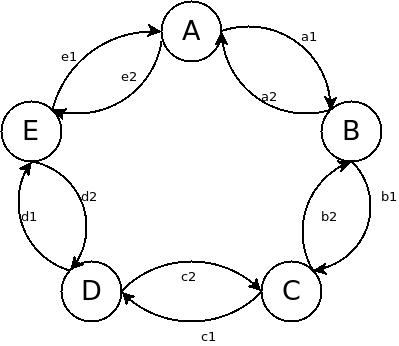
\includegraphics[width=0.5\textwidth]{Imagen/ejercicio5tema3.jpg}
	\caption{Anillo STM-16}
	\end{figure}
	\begin{tabular}{c|c|c|c|c|c|c|c|c|c|c|c|c|c|c|c|c|}
		   & 1  & 2  & 3  & 4  & 5  & 6  & 7  & 8  & 9  & 10 & 11 & 12 & 13 & 14 & 15 & 16 \\\hline
		a1 &    &    &    &    &    &    &    & EB & AD & AD & AD & EC & EC & AC &    &    \\\hline
		a2 &    &    &    &    &    &    &    & BE & DA & DA & DA & CE & CE & CA &    &    \\\hline
		b1 & BC & BC &    &    &    &    &    &    & AD & AD & AD & EC & EC & AC &    &    \\\hline
		b2 & CB & CB &    &    &    &    &    &    & DA & DA & DA & CE & CE & CA &    &    \\\hline
		c1 &    &    &    & CE & CE & CA &    &    & AD & AD & AD & EC & EC & AC &    &    \\\hline
		c2 &    &    &    & EC & CE & AC &    &    & DA & DA & DA & CE & CE & CA &    &    \\\hline
		d1 &    &    &    &    &    &    &    &    &    &    &    &    &    &    &    &    \\\hline
		d2 &    &    &    &    &    &    &    &    &    &    &    &    &    &    &    &    \\\hline
		e1 & DA & DA & DA &    &    & CA &    & EB & AD & AD & AD & EC & EC & AC &    &    \\\hline
		e2 & AD & AD & AD &    &    & AC &    & BE & DA & DA & DA & CE & CE & CA &    &    \\\hline
	\end{tabular}
\end{exercise}
\begin{exercise}[6]
	Decodifique y determine la secuencia de alineamiento del interfaz U de un acceso primario en el que se recibe la siguiente colección de bits sabiendo que los primeros 8 bits del canal número 3 son 00001000: ···-0+0-+-00+-000+-00-00+000-+00-+00+0-000-+-+000+-+-···\\
	Lo primero vemos que al tratarse de un acceso primarioel mensaje está codificado en HDB3. El primer paso para resolver el ejercicio será la decodificación completa. Hay que tener en cuenta que cada vez que se rompa la alternancia de más y menos este el bit que la rompe será un cero. Asimismo, los tres bits anteriores también serán ceros.\\
	Mensaje descodificado: 10101110011000100000010001100100000100001110000111. Después de esto solo queda identificar los primeros 8 bits del canal 3 y de ahí contar 16 bits hacia atrás para encontrar los 8 bits de alineamiento. Se puede ver que existen dos posibles inicios del canal 3. El primero no puede ser, ya que no está suficientemente retrasado para incluir la trama de alineamiento en el mensaje descodificado. El segundo, en cambio si, podemos ver que la trama lleva una alineación como la siguiente: 00110001.
\end{exercise}
\begin{exercise}[7]
	Se desea establecer un enlace RDSI entre dos ciudades que distan 35km e intercambian un tráfico de 102E, con el objetivo de que la probabilidad de pérdida de llamadas de los usuarios sea inferior al 1\%. Los circuitos necesarios se implementarán mediante multiplex MIC de norma europea. Se ha decidido tener una línea de postes con un único cable 25-CEF (25 pares con aislamiento de plástico de calibre 0.91 mm), que se utilizará para la transmisión en BF y MIC, cuyos parámetros a la frecuencia de 1024 kHz son:
	\begin{itemize}
		\item Atenuación: $12\sfrac{dB}{km}$
		\item Atenuación de diafonía para una longitud de 1km: 15dB
	\end{itemize}
	Se estima que el ruido térmico y de intermodulación se pueden despreciar frente a la diafonía y que la atenuación de diafonía en función de la longitud del cable se puede expresar como:
	\[A_D(L)=A_D(L_0)+10log(\frac{L}{L_0}\]
	Para las secciones de regeneración, se dispone de regeneradores de 42 dB de ganancia, con una sensibilidad a la diafonía de 18 dB. Se reservarán tres pares de cable para supervisión. El departamento de contabilidad de la compañía suministra los siguientes datos (miles de €):
	\begin{center}
	\begin{tabular}{c c c}
		\hline
		\textbf{Concepto} & \textbf{Mano de obra} & \textbf{Materiales}\\\hline
		Mux digital (mux y demux) & 3 & 5,5\\
		ETL (tx y rx) & 1,5 & 1,8\\
		Tendido de 1km de cable & 0,35 & 0,5\\
		Repetidor intermedio bidireccional & 1 & 0,8\\
		Instalación de 1km de línea de postes & 0,6 & 0,12\\\hline
	\end{tabular}
	\end{center}
	Las secciones de regeneración se dispondrán siguiendo el esquema de la siguiente figura:
	\begin{figure}[htp]
	\centering
	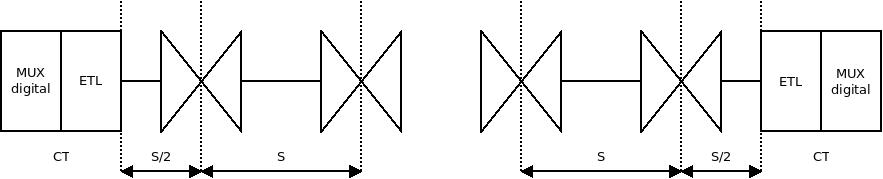
\includegraphics[width=\textwidth]{Imagen/ejercicio7tema3.jpg}
	\caption{esquema de las secciones de regenaración}
	\end{figure}
	Nota: Para el cálculo de la diafonía se puede suponer que las señales del sistema perturbador y del perturbado tienen la misma potencia.\\
	Se pide:\\
	\textbf{1.} Determine el número de multiplex MIC necesarios\\
	\[N_{MIC}=\frac{B^{-1}(A_o,P_B)}{30}=4\text{ multiplex MIC}\]
	\textbf{2.} Determine la longitud máxima de los tramos cuya atenuación puede ser compensada por los regeneradores\\
	\[S_{MAX}=\frac{42dB}{12\sfrac{dB}{km}}=3,5km\]
	Hay que poner un regenador cada menos de 3,5km para que la señal se pueda recuperar.
	\textbf{3.} ¿Cuántos pares son susceptibles de ser explotados en BF?\\
	\[N_{BF}=N_{pares}-2*N_{MIC}-N_{supervision}=25-2*4-3=14\text{ pares para BF}\]
	\textbf{4.} Determine la longitud de la sección de regeneración\\
	\begin{gather*}
		A_D(S_{min})\geq S_D\\
		A_D(L)=A_D(L_0)+10log(\frac{S_{min}}{L_0}\geq 18dB\\
		S_{min}\geq 1.99km\\
		1.99km\leq S \leq 3.5km
	\end{gather*}
	Elegiremos un valor de span entre el mínimo de 1.99km y el máximo de 3.5km. Para reducir coste intentaremos elegir valores cercanos al máximo, 3.5km.
	\textbf{5.} Inversión inicial\\
	Si elegimos usar el valor de span máximo obtendríamos una inversión inicial de 96 millones de euros, Si en cambio cogemos el valor mínimo el precio ascendería a los 109 millones de euros.
	\[Precio=2*Mux+2*ETL+35*(cable+postes)+\frac{35km}{S}repetidor\]
\end{exercise}
\begin{exercise}[8]
	En las figuras (a) y (b) se muestran dos esquemáticos de sistemas ópticos, válidos para WDM, se le pide que calcule las pérdidas totales por inserción entre
\begin{enumerate}
	\item Entrada y salida de figura (a)
	\item A y B en el ADM óptico de la figura (b)
	\item A y C en el ADM óptico de la figura (b)
\end{enumerate}
\begin{center}
\begin{tabular}{c c}
	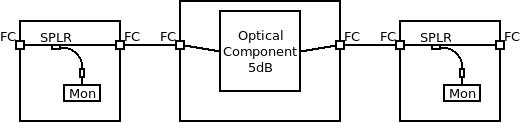
\includegraphics[width=0.4\textwidth]{Imagen/ejercicio8tema3a.jpg}
	& 
	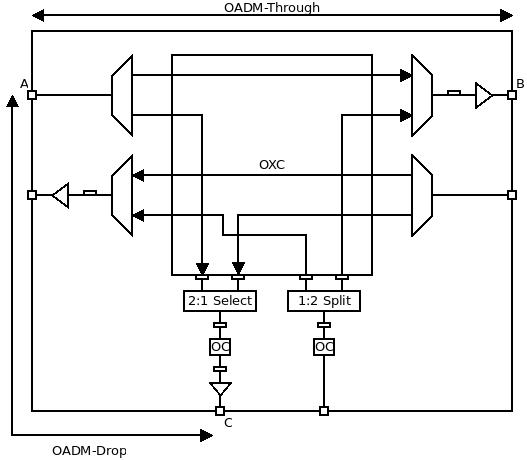
\includegraphics[width=0.4\textwidth]{Imagen/ejercicio8tema3b.jpg} \\
	Figura (a) & Figura (b)
\end{tabular}
\end{center}
Sabiendo que cada dispositivo monitor (Mon) añade 0.6 dB de pérdidas, y el resto de parámetros se muestran en la tabla siguiente:
\begin{center}
\begin{tabular}{c | c}
\hline
	\textbf{Componente} 	& \textbf{Valor}\\\hline
	Fibra Monomodo			& 0,1dB/km\\
	Conector de Fibra		& 0,4dB\\
	Conector Multifibra		& 0,5dB\\
	Empalme (Splice)		& 0,2dB\\
	Mux óptico				& 1dB/canal\\
	Demux óptico			& 1dB/canal\\
	OXC (through)			& 0,5dB\\
	OXC (drop)				& 2dB\\
	Divisor (splitter)		& 3dB\\
	Tap						& 0,2dB\\
	Selector 2:1			& 3dB\\
	Filtro					& 0,5dB\\
	Ganancia Amplificador	& 6dB\\
	Convertidor de $\lambda$ (OC)	& 1dB\\\hline
\end{tabular}
\end{center}
\textbf{1. Entrada y salida de la figura (a)}\\
\[L_{AB}=6FC+2SPLR+5dB+2Mon=14,6dB\] 
\textbf{2. A y B en el ADM óptico de la figura (b)}\\
\[L_{AB}=2FC+1Demux+1OXC(through)+1Mux+1Splice-G_{AO}=-3.5\sfrac{dB}{canal}\]
\textbf{3. A y C en el ADM óptico de la figura (b)}\\
\[L_{AC}=2FC+1Demux+1OXC(Drop)+1Selector+1OC+3Splice-G_{AO}=2,4\sfrac{dB}{canal}\]
\end{exercise}
\begin{exercise}[9]
	Se desea calcular la potencia total recibida en un sistema DWDM en el que hay 40 canales, y que se transmite en una fibra mono-modo que tiene una atenuación de 0.1dB/km, y una dispersión cromática de 0.5ps/nm·km y una dispersión por polarización de 0.12ps/$\sqrt{km}$. El sistema cuenta con 40 canales en la banda C, separados 100nm, y cada uno a 10Gbps. El transmisor, un laser, es capaz de acoplar 0dBm a la fibra con una precisión de f±20nm. Como receptor se tiene un diodo APD, que tiene una sensibilidad de -33dBm para obtener una BER de $10^{-9}$ . Las pérdidas del multiplexor/demultiplexor de paso son 7dB, mientras que las del de extracción son de 8dB. El amplificador tiene una ganancia de 0dB, en cada empalme se pierden 0.2dB y en cada conector 0.5dB. En los 80km de longitud del sistema, hay 4 conectores, 10 empalmes y se espera que en el futuro pueda haber 4 empalmes más. Además, se dejan 2dB de margen para otras degradaciones en el sistema.\\
1. Calcular la potencia recibida\\
2. ¿Permite el sistema margen para futuros empalmes?\\
3. ¿Cumple las especificaciones?
\end{exercise}
\begin{exercise}[10]
	Calcule el span de un sistema en el que se utiliza fibra mono-modo cuya atenuación son 0,1dB/km y su dispersión cromática son 21ps/nm·km con modulación NRZ. El láser es del tipo DFB y es capaz de acoplar a la fibra una potencia de 0dBm. Para compensar la dispersión cromática se utilizan DCF, que no obstante dejan una dispersión residual de 2ps/nm·km añadida. La sensibilidad cromática de estos DCF es de 50ps/nm, y su sensibilidad en recepción es de -1.32 dBm, pero cuentan con una etapa amplificadora de 3dB a su salida. Las pérdidas introducidas por los conectores es de 0,4dB por conector.\\
Nota: Para cada DCF se necesitan dos conectores.\\
El primer paso será determinar el número máximo de DCF's que se pueden poner pudiendo recuperar la señal al otro lado.
\[N_{DCF}=\frac{S_{DC}}{DC_{residual}}=\frac{50\sfrac{ps}{nm}}{2\sfrac{ps}{nm}}=25DCF\]
\end{exercise}